%{{{ setup
\documentclass[conference]{IEEEtran}
\usepackage{amsmath,url,color,algorithm, algorithmic, amssymb}
\usepackage{setspace, graphicx}
\usepackage[x11names,rgb]{xcolor}
\usepackage{tikz}
\usetikzlibrary{snakes}
\usetikzlibrary{arrows}
\usetikzlibrary{shapes}
\usetikzlibrary{backgrounds}
\usetikzlibrary{patterns}
\usepackage[cm]{fullpage}
\usepackage[scriptsize,tight]{subfigure}
\usepackage[
pdftitle={title},
pdfcreator={pdftex},
pdfsubject={SCXY 2009},
hyperindex = {true},
colorlinks = {true},
linkcolor = {blue},
citecolor = {blue}
]{hyperref} 
\graphicspath{{figs/}}

\input macros.tex
\newcommand{\peq}{+\!\!=}

\begin{document}

\title{Parallel Fast Gauss Transform}  


\author{\IEEEauthorblockN{Rahul Sampath}
\IEEEauthorblockA{Oak Ridge National Laboratory\\
       Oak Ridge, TN 37831\\
       Email: sampathrs@ornl.gov} 

\and
\IEEEauthorblockN{Hari Sundar}
\IEEEauthorblockA{Siemens Corporate Research \\
       Princeton, NJ 08540 \\
       Email: hari.sundar@siemens.com}

\and
\IEEEauthorblockN{Shravan Veerapaneni}
\IEEEauthorblockA{New York University \\
       New York, NY 10012 \\
       Email: shravan@cims.nyu.edu}
}
\date{}
\maketitle

\begin{abstract}
We present a fast parallel algorithm to compute the sum of $N$ Gaussians at $N$ points in an optimal $\bigO(\frac{N}{n_p})$ time on $n_p$ processors. Our implementation is based on the plane-wave representation of the kernels which permits diagonal translation. We present a new algorithm for translation that minimizes work and memory loads compared to previous schemes.
Computing the transform to six-digit accuracy at 120 billion points took 185 seconds on 4096 cores of Jaguar. 
\end{abstract}

\section{Introduction}  \label{s:intro}
Gauss transform is one of several discrete spatial transforms of the form 
%
\beq F(x_j) = \sum_{k=1}^N \kernel f_k \quad \text{at} \quad \{ x_j \, | \, j = 1,...,M \} \, , \label{gt} \eeq
\[\text{where} \quad x_j, y_k \in \mathbb{R}^d. \]
%
where the kernel $G_\delta$ is smooth, exponentially decaying in both physical and Fourier domain. The parameter $\delta$ controls how rapidly the kernel decays.  
In the Gauss transform case, $\kernel = e^{-\frac{\|x_j - y_k\|^2}{\delta}}$.  We call the points $x$ as targets and $y$ as sources.  

Discrete sums of the form (\ref{gt}) are encountered in a variety of disciplines including computational physics, machine learning, computational finance and computer graphics. Computing these sums directly takes $\bigO(NM)$ time and is not feasible for large scale problems. Starting from the earlier work of Greengard and Strain \cite{fgt}, several sequential algorithms have been proposed (e.g.,  \cite{greengard98, duraiswami03, fggt}) to reduced the cost to an optimal $\bigO(N+M)$. However, to our knowledge, there have been no parallel implementations to date. 

\textbf{Contributions.}
\begin{itemize} 
\item We propose a new sequential and parallel algorithm to compute (\ref{gt}) when the sources are distributed on arbitrarily adaptive grids. Our scheme is an extension of the tree-splitting scheme proposed in \cite{veerapaneni08} for computing continuous Gauss transforms. 
\item We present a novel sequential and parallel translation scheme for the plane wave expansions.
This scheme particularly minimizes the computational cost and memory requirements 
when the source distribution is highly nonuniform. 
\item 
\end{itemize}


\section{Overview of FGT}
For simplicity, we assume that the points are uniformly distributed and that they reside within a unit cube.
The design of fast algorithms for (\ref{gt}) is strongly dependent on three independent parameter viz., number of sources $N$, the bandwidth $\delta$ and desired accuracy $\epsilon$. A Gaussian centered at a source location interacts with targets that are within its support. If there are fewer targets than a threshold value $n^*$, we use a simple {\em truncation algorithm}, otherwise, we use a {\em expansion algorithm}. The threshold  value depends on all three independent parameters and we will discuss its choice after introducing both algorithms. 

\subsection{Truncation algorithm} 
Since the kernel in (\ref{gt}) decays exponentially, we can simply truncate the sum to
%
\beq F(x_j) = \sum_{y_k \in \mathcal{I}[x_j]} \kernel f_k \eeq
%
where $\mathcal{I}[x_j]$ is the interaction list which includes all the sources that are within a distance $\sqrt{\delta \ln (1/\epsilon)}$. Beyond this distance, a Gaussian centered at $x_j$ decays below $\epsilon$. The complexity of this algorithm is $\bigO(N \sqrt{\delta \ln(1/\epsilon)})$. This is a common technique used in the graphics community. When $\delta$ is large and/or high accuracy is required, the cost of this algorithm grows quadratically.  

\subsection{Expansion algorithm}
There are two variations of FGT: one based on hermite expansion \cite{fgt} and another based on plane-wave expansion \cite{greengard98}. The former has lower expansion costs while the latter has lower translation costs. The latter version is further improved in \cite{fggt} for volumetric data. Our implementation is based on \cite{fggt} and we summarize it here. 

The central is the finite-term plane-wave representation of the kernel,
\beq G_\delta(\norm{x_j - y_k}) \approx \sum_{|k| \leq p} \hat{G}(k) e^{i \lambda k \cdot (x_j - y_k)}, \quad \lambda = \frac{L}{p\sqrt{\delta}}\eeq
where $k = (k_1, k_2, k_3)$ and the parameters $p$ and $L$ are determined by the required precision. $\hat{G}$ is the discrete Fourier transform of the kernel. For the Gaussian kernel, we have 
\beq \hat{G}(k) = \left(\frac{L }{2p\sqrt{\pi}}\right)^3 e^{-\frac{\lambda^2 |k|^2 \delta}{4}}.\eeq

The algorithm begins by partitioning the domain into uniform boxes of size $\sqrt{\delta}$ each. A Gaussian located at the center of a box $B$ decays below $\epsilon$ beyond a fixed number of boxes. We call these boxes the interaction list of $B$, denoted by $\mathcal{I}[B]$. 

In the fast algorithm, a target point $x$ receives information from a source point $y$ via 
\begin{enumerate}
\item{S2W:} The influence of all the sources in a box $B$ is condensed into a plane wave expansion.
            \beq w_k = \eeq
\item{W2L:} The plane wave expansion of each box is transmitted to all the boxes in its interaction list. 
            \beq v_k = \eeq
\item{L2T:} The local plane wave expansion is evaluated at the target locations. 
\end{enumerate} 

When there are significantly more number of sources in each box, it is easy see why we


%

\subsection{A novel scheme for translation} 
Once the wave expansions are formed at all the FGT boxes, the next step is to form each of their local expansions. Since the FGT boxes are of size $\bigO(\sqrt{\delta})$, only a fixed number of surrounding boxes contribute to the local expansion of a box $B$. We shall call these set of boxes as its {\em interaction list}, denoted by $\mathcal{I} [B]$. A {\em direct scheme} forms the local expansion by simply visiting all the boxes in $\mathcal{I}[B]$ and translating their wave expansions. After initializing the local expansions $\{ v_k \quad \forall \quad |k| \leq p \}$ to zero, the pseudo-code for the direct scheme is:
%
{\tt
\begin{algorithmic}
\STATE {\sc Direct scheme}
  \FOR {each $C \in \mathcal{I}[B]$}
           \STATE $ v_k^B \quad += e^{i z_k \cdot(c^B - c^C)/\sqrt{\delta}} w_k^C \quad \forall \quad |k| \leq p$
       \ENDFOR
\STATE
\end{algorithmic}
}
%
Assuming the size of $\mathcal{I}[B]$ is $K^3 - 1$, this algorithm requires $\bigO(K^3 p^3 N_B)$ work to form local expansions at all the boxes. 
%
\input sweep.tex

Based on the cost of the expansion based algorithm, we 

{\tt
\begin{algorithmic}
\STATE
  \IF {$N \sqrt{\delta \ln \left( \frac{1}{\epsilon} \right)} < \frac{1}{2}(2p)^3 $}
     \STATE Use truncation algorithm 
  \ELSE 
     \STATE Use expansion based algorithm
  \ENDIF
\STATE
\end{algorithmic}
}



\section{Nonuniform distributions} 

{\bf MOTIVATION}

In the uniform distribution case, we can precisely estimate the threshold $n_{th}$ that decides whether one should use the truncation algorithm or the expansion based algorithm. However, when the source and target distributions are highly nonuniform, as is the case in most practical applications, it is not straightforward. For example, when we superimpose a regular grid structure of FGT on a nonuniform distribution, some boxes will have lot of points while some are almost empty. 

%

{\bf OCTREES}
We assume sources and targets are the same for simplicity. We also assume that the octree is constructed so that there are no more than a fixed number of points in each leaf node. 

\begin{algorithm}[!h]
\caption{{\em Tree Splitting}}
{\tt
\begin{algorithmic}
\STATE
  \FOR {each leaf node $\ell$}
      \IF {$|\ell| > \sqrt{\delta}$}
          \STATE assign $\ell$ to $T_d$ (direct or truncation based)
      \ELSE
          \STATE assign $\ell$ to $T_e$ (expansion based)
      \ENDIF
  \ENDFOR
\STATE
\end{algorithmic}
}
\end{algorithm}


\begin{algorithm}[!h]
\caption{\em FGT on a split tree}
%\label{a:ofgt}
{\tt
\begin{algorithmic}
\STATE
%\STATE {\sc FGT on a split Octree}
  \FOR {each $\ell \in T_e$}
      \STATE (S2W) Add contribution of point in $\ell$ to the FGT box it belongs
  \ENDFOR
  \STATE
  \STATE (W2L) Form local expansions using sweeping
  \STATE 

  \STATE {\sc Evaluate the effect of all sources in $T_d$}
  \FOR {each $\ell \in T_d$}
       \FOR {$x \in \ell$}
          \STATE Add contribution of $x$ to all the target boxes (in $T_e$) and target points (in $T_d$)     
       \ENDFOR  
  \ENDFOR
  
  \STATE 
  \STATE {\sc Evaluate the effect of all sources in $T_e$}
     \FOR {each FGT box $B \in T_e$}
        \STATE Use local expansion for target points within $B$ 
        \STATE
        \STATE Use wave expansion for target points in $T_e$ that are within its interaction list
     \ENDFOR  
\STATE
\end{algorithmic}
}
\end{algorithm}

{\em [In the parallel case, the interaction between $T_d$ and $T_e$ can be done while processors are communicating other info.] }




\begin{figure}[htp]
\begin{center}
  \subfigure[]{\label{fig:Grid1}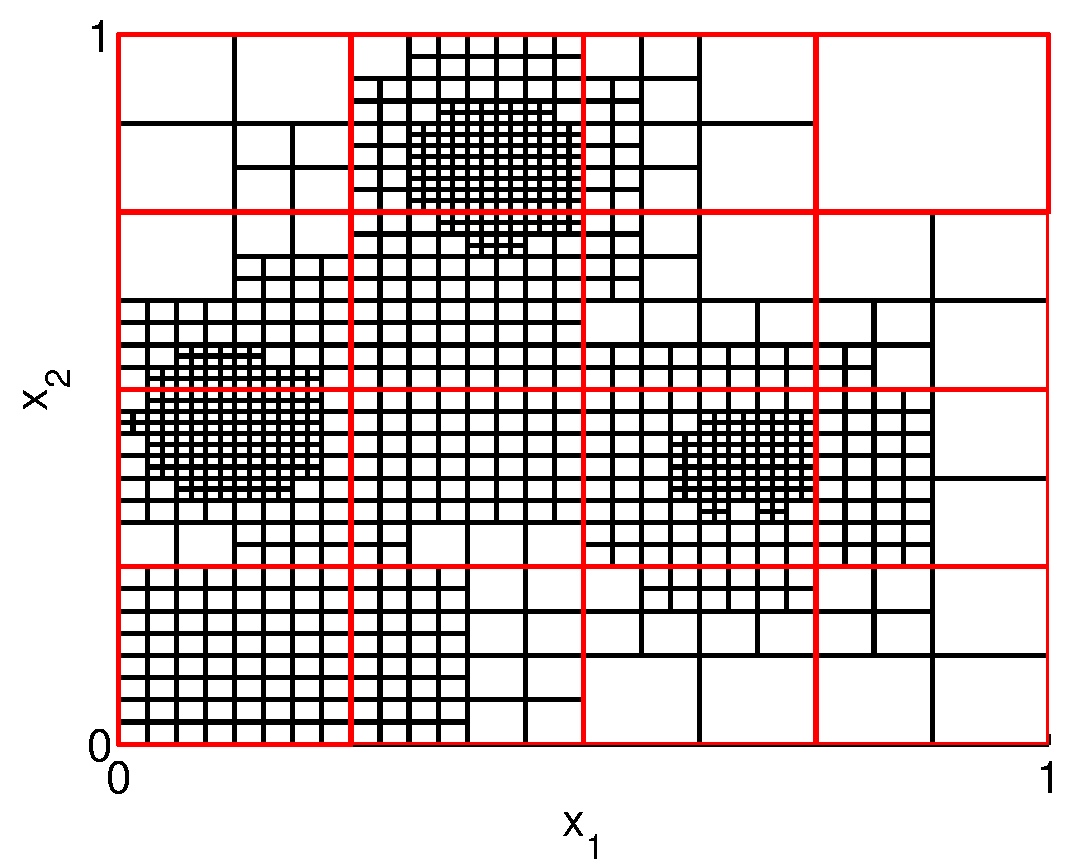
\includegraphics[scale=0.32]{Grid1}}
  \subfigure[]{\label{fig:Grid2}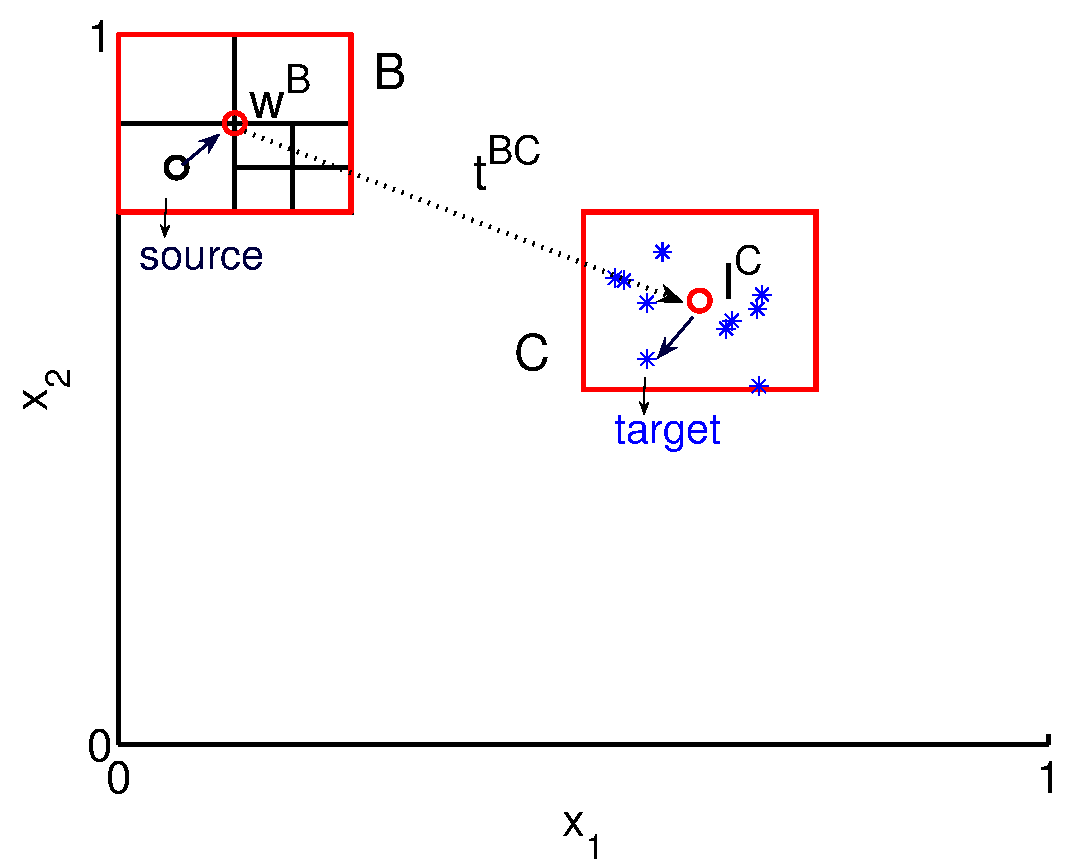
\includegraphics[scale=0.32]{Grid2}}  
 \end{center}
\caption{\em Here we illustrate one of the main steps involved in
  FGT. a) The leaf nodes (shown in black) of the given quadtree
  are assigned to regular boxes (shown in red). The size of the boxes
  is chosen so that each box corresponds to a node at some level of
  the quadtree. b) At a source box $B$, the influence of all  
  the constituent leaf nodes is encoded in the wave expansion
  $\mb{w}^B$. The translation operator  
  $\mb{t}^{BC}$ transfers the wave expansion of $B$ to the target box
  $C$. At $C$, the influence of all the source
  boxes in $\mci[C]$ is encoded in the local expansion $\mb{l}^C$.
  Finally, $\gausst f$ at a target that belongs to $C$ is given by
  $<\mb{l}^C, \mb{v}^C(\mbx)>$.}\label{fig:Grid}
\end{figure}
%
\begin{figure}[htp]
\begin{center}
  \subfigure[$Q$]{\label{fig:Qtree0}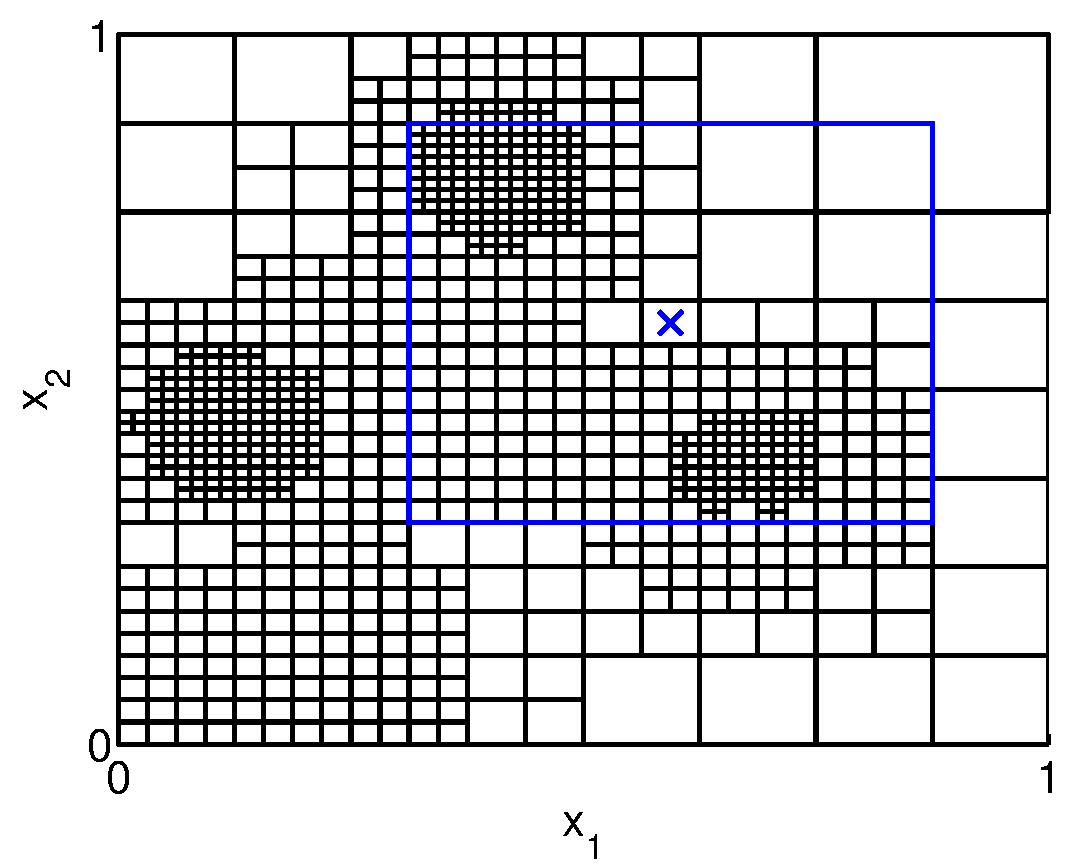
\includegraphics[scale=0.3]{Qtree0}}
  \subfigure[$Q_{\text{Direct}}$]{\label{fig:Qtree1}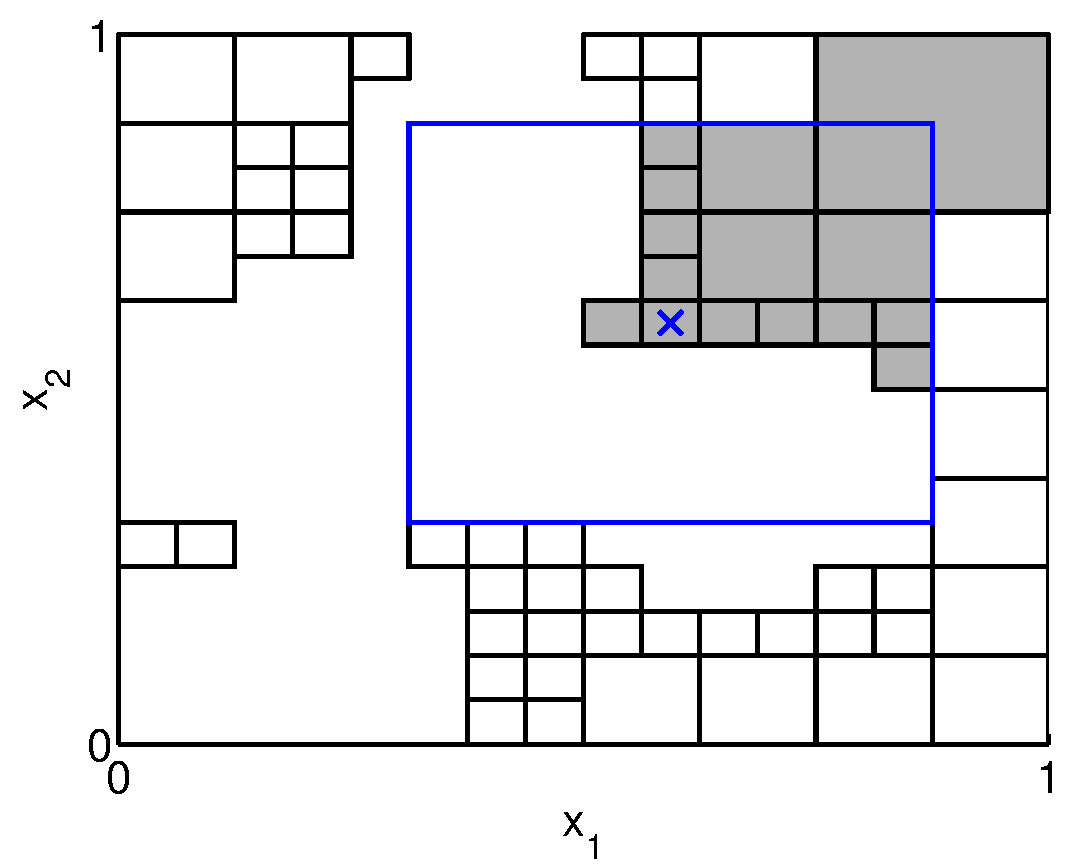
\includegraphics[scale=0.3]{Qtree2}}
  \subfigure[$Q_{\text{Expand}}$]{\label{fig:Qtree2}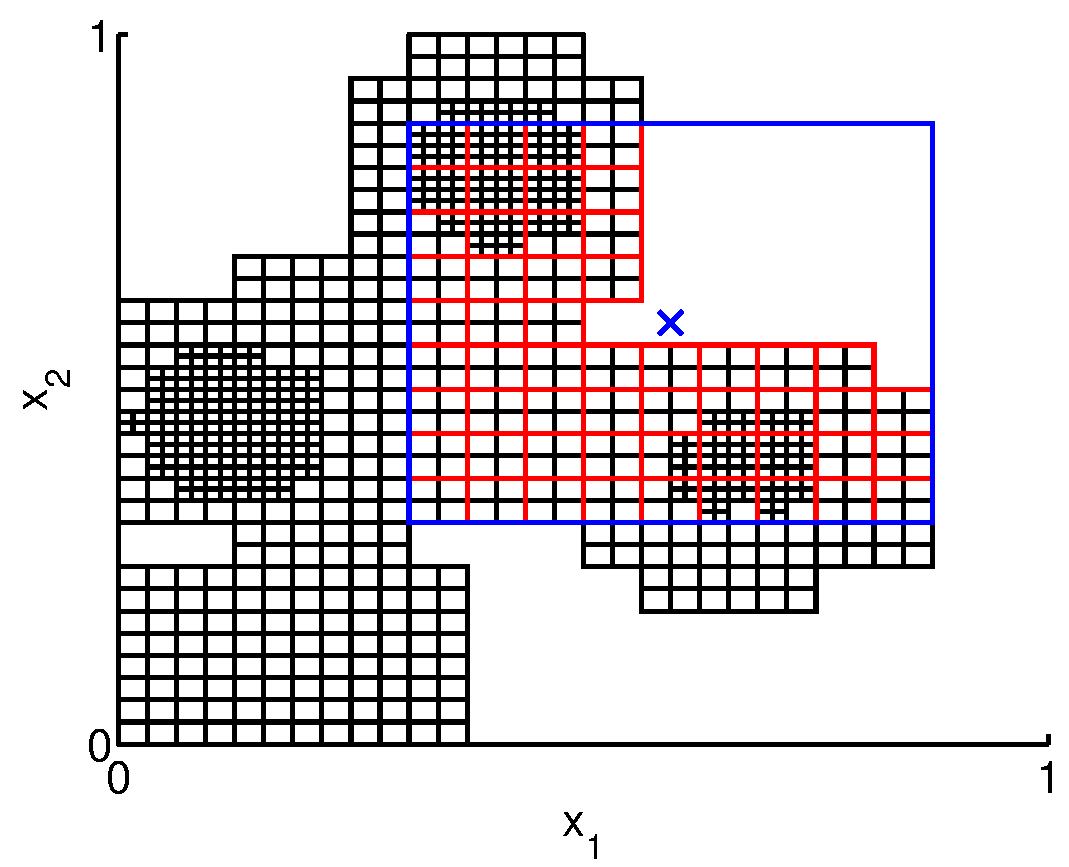
\includegraphics[scale=0.3]{Qtree1}}
  \end{center}\caption{\em In this figure we illustrate the tree
  splitting that we use in CFGT to obtain an algorithmic complexity
  that is independent of the value of $\delta$.  Subfigure (a) shows
  the quadtree, a target $\mbx$, and the support of the Gaussian
  centered at $\mbx$ (blue box). For this $\delta$, we can observe
  that a direct evaluation would be expensive because we have to loop
  through all the leaf nodes within the support. A kernel expansion
  based approach would also be expensive because it generates too many
  boxes. Hence, for optimal complexity, we split the tree into
  two parts. Subfigure (b) shows the tree with the size of leaf nodes
  being greater than $r_b$. To evaluate the Gauss transform at a point
  $\mbx$, we just need to visit the leaf nodes in the support of the
  Gaussian (the shaded ones). There can be a maximum of $(2n+1)^2$ of
  such leaf nodes. Subfigure (c) show the tree with the size of leaf
  nodes being smaller or equal than $r_b$. In this tree we use the
  kernel expansion-based algorithm. Instead of visiting all the leaf
  nodes within the support, we only have to gather the wave expansion
  of the source boxes (red boxes) that are within the support. The
  number of these source boxes is bounded from above by
  $(2n+1)^2$. }\label{fig:qtree_split}
\end{figure}

\section{Results}

\begin{table}[h!]
\small
\begin{center}
\begin{tabular}{|c|c|c|c|c|}
\hline
Operation & Max. Time & Avg. Time & Max. Flops & Avg. Flops\\
\hline
S2W & & & & \\
\hline
W2L & & & & \\
\hline
L2T & & & & \\
\hline
Total & & & & \\
\hline
\end{tabular}
\end{center}
\caption{{\rm {\footnotesize Timings on 37,268 ($32^3$) processors on Jaguar. The point distribution is uniform random, the parameter $\delta = 8 \times 10^{-4}$ and precision $\epsilon = 10^{-6}$}}. Each processor has a million points.}}
\label{t:scaling}
\end{table}

\begin{figure*}
	\begin{center}
%		\subfigure[uniform]{\scalebox{1}{\input{figs/uniform_fixed.tex}}}
%		\gap
%		\subfigure[ellipse]{\scalebox{1}{\input{figs/ellipse_fixed.tex}}}
	\end{center}
\caption{Strong scaling on Jaguar. The problem size is fixed to 1 billion points and the parameters are the same as defined in Table \ref{t:scaling}. [Rahul: Try varying the num. of processors from 16 to atleast 8192]}
\label{f:fixed}
\end{figure*}

\begin{figure*}
	\begin{center}
%		\subfigure[uniform]{\scalebox{1}{\input{figs/uniform_iso.tex}}}
%		\gap
%		\subfigure[ellipse]{\scalebox{1}{\input{figs/ellipse_iso.tex}}}
	\end{center}
\caption{Weak scaling on Jaguar. Number of points per proceesor is fixed at 1 million (so $N = 10^6 \times n_p$) and the parameter $\delta = \frac{10}{N^{1/3}}$. [Rahul: Try varying the num. of processors from 16 to atleast 8192]}
\label{f:iso}
\end{figure*}



\section{Conclusions}

%\texbf{Periodic kernels.} If the kernel $G_\delta(x,y)$ is periodic in the unit cube, the fast Fourier transform (FFT) can be used for the fast computation of (\ref{gt}) assuming regular grids. 
Several acceleration techniques for forming and evaluating plane wave expansion were introduced in \cite{fggt}. We will incorporate these in our final submission. When the sources come from a tensor product grid in each octant, the expansion constants can be reduced from exponential to linear in dimension. In the sequential case, this speed-up will make the cost of the algorithm comparable to that of fast Fourier transform (FFT). Since the parallel performance of FFT has been sub-optimal till date, we believe that our parallel FGT would be the method of choice even for regular grids. 


{\em
A few assumptions to simplify our implementation: 
\begin{enumerate}
\item Each processor has finite number of FGT boxes. If we also care for the contrary, we would have a box that spans across processors and hence S2W and L2T also need to parallelized. Not a big deal, but simplifies our job for now. 
\item We will assume that $\delta = 2^{-n}$ for some even number n and FGT box size $h = \sqrt{\delta}$. This will help us in reducing book-keeping: otherwise, in the octree case, we will have FGT boxes cutting across leaf nodes. 
\end{enumerate}
}


\bibliography{sc10}
\bibliographystyle{siam}
\end{document} 
